\documentclass[a4paper,10pt]{article}

% -----------------------------
% Pacchetti base
% -----------------------------
\usepackage[utf8]{inputenc}      % codifica input
\usepackage[T1]{fontenc}         % codifica font
\usepackage{lmodern}             % font moderno
\usepackage{xcolor}               % colori
\usepackage{geometry}             % margini comodi
\geometry{margin=2cm}
\usepackage{float}                % per [H]
\usepackage{graphicx}             % immagini
\graphicspath{{images/}{Courses/images/}} % cartelle immagini
\usepackage{tikz}                 % TikZ
\usepackage{pgfplots}             % grafici
\usetikzlibrary{pgfplots.statistics}
\pgfplotsset{compat=1.18}
\usepackage{amsmath, amssymb, amsfonts, amsthm} % matematica
\usepackage{tocloft}              % sommario personalizzato
\usepackage{listings}             % codice
\usepackage[colorlinks=true, linkcolor=black]{hyperref} % link
\usepackage{minted}

% -----------------------------
% Codice con colori
% -----------------------------
% Minted (richiede -shell-escape)
\usepackage{minted}
\setminted{fontsize=\small, breaklines, frame=single, framesep=3mm}

% Ambiente per Python
\newenvironment{pythoncode}
{\VerbatimEnvironment\begin{minted}[linenos, bgcolor=gray!10]{python}}
{\end{minted}}

% Ambiente per R
\newenvironment{rcode}
{\VerbatimEnvironment\begin{minted}[linenos, bgcolor=blue!5]{r}}
{\end{minted}}

% -----------------------------
% Comandi personalizzati
% -----------------------------
\newcommand{\ra}{\ensuremath{\rightarrow}}
\newcommand{\la}{\ensuremath{\leftarrow}}
\newcommand{\lra}{\ensuremath{\leftrightarrow}}
\newcommand{\Ra}{\ensuremath{\Rightarrow}}
\newcommand{\La}{\ensuremath{\Leftarrow}}
\newcommand{\Lra}{\ensuremath{\Leftrightarrow}}

% Highlight veloce
\newcommand{\hl}[1]{\textbf{\textcolor{red}{#1}}}

% -----------------------------
\begin{document}

\title{Cheatsheet}
\author{Libero Biagi}
\date{\today}
\maketitle

\section*{Intro}
This is a general cheatsheet where I will try to put all the coding, the formulas, the terminology and the possible exercises that might be useful for the exams.

\tableofcontents

% Inclusione dei capitoli
\section{Data Mining}
\subsection{Theory}

\subsubsection{Introduction}

Fernando Becao presents himself and the tutor.

Fernando Becao asks us why we weren't at the party.

We study about supervised and unsupervised learning.

Exam + project.

Exam is 55\% of the final grade

Project is 45\% and is divided into

\begin{itemize}

\item Deliverable 1 -> 30\% by November 4th
\item Deliverable 2 -> 60\% by January 3rd
\item Discussion -> 10\%
\end{itemize}

Both exam and project will expire after the year


\subsubsection{Context}

Random debate about things

We need to find relevant data to reduce computation and improve the quality of works

\vspace{10pt}

\textbf{Big Data} -> we simplify datasets that are too big for normal processing. From big data into mean datasets

Big data characteristics:
\begin{itemize}
    \item \textbf{Volume:} big data are big
    \item \textbf{Velocity:} Big data technology allows databases to process and analyze data while it is being generated
    \item \textbf{Variety:} Big data can be a mixture of structured, unstructured and semi-structured data. To solve this problem Big Data is flexible
\end{itemize}

Some information about AI, ML and Data Science.

\vspace{10pt}


\textbf{AI:} Making things that show human intelligence. Automatize human tasks.

\vspace{10pt}

\textbf{Machine Learning:} Approach AI using systems that can find patterns from data and examples. ML systems learn by themselves. We can see them as a sort of subset of AI or a way towards AI 

\vspace{10pt}

\textbf{Data Science:} the study of where information comes from and how to turn it into a valuable resource.
\vspace{10pt}


\textbf{Data Science vs Data Mining}
\vspace{10pt}

Data science is a set of principle that guide the extraction of information from data. We try to view problems from a data perspective.

\vspace{10pt}

Data mining on the other hand is the extraction of knowledge from data via the use of algorithms.


\vspace{10pt}


Find/build attributes is very important. Basically the properties of the things that we are studying have to be selected or preprocessed.

\vspace{10pt}

After the construction of the features a ML model can learn how to divide the instances on an hyperplane. This can be used to make predictions. Recall that a model will predict only based on the class that it was trained on.

\vspace{10pt}

Is very important to use the relevant and appropriate features. More features can mean more possibility of discriminating between the classes. 

\vspace{10pt} Typically we use labeled examples, enough data and clear cut definitions.

\vspace{10pt}

If our models try to attribute a label we have supervised learning. Future examples will get a prediction.


\vspace{10pt}


To build features we use data warehouse and ETL (extract, transform and load). Recall that we can transform every relational schema into a table (at least with SQL).

\vspace{10 pt}

Minimum information to identify a costumer:
\begin{itemize}
    \item Transaction number
    \item Date and time of transaction
    \item Item purchased
    \item Price
    \item Quantity purchased
    \item A table that matches product code to its name, subgroup code to name, product group code to group name.
    \item Product taxonomy to link product code to subgroup code and product subgroup code to product group code.
    \item Card ID
\end{itemize}

Consistent behaviors are easier to analyze. To found the level of consistency i can use the standard deviation and I can remove the outliers.

\vspace{10pt}

We can also look at relevant variables like:
\begin{itemize}
    \item Recency
    \item Frequency
    \item Monetary value
    \item Average purchase
    \item Most frequent store
    \item Average time between transactions
    \item Standard deviation of transactional interval
    \item Costumer stability index
    \item Relative spend on each product
\end{itemize}

\textbf{Canonical tasks in data mining}

If we want to classify new data from a decision criterion previously learned we talk about \textbf{Supervised learning}

\vspace{10pt}

If we want to summarize a data set we talk about \textbf{Unsupervised learning}

\vspace{10pt}

\textbf{Supervised learning:}
\begin{itemize}
    \item Classification
    \item Regression
\end{itemize}

\textbf{Unsupervised learning:}
\begin{itemize}
    \item Clustering
    \item Visualization
    \item Association
\end{itemize}

\vspace{20pt}

In our datasets the features are the columns while the rows are the instances

\vspace{20pt}

\textbf{Clustering} -> We plot the instances on a hyperplane and we try to group them by distance, we can have different plots 

\textbf{Association rules} -> based on our data we can use the transactions to find some rule to infer costumer routine. We use confidence, support, lift and so on.

\textbf{Visualization} -> n-D data can be difficult to visualize so we can flatten them into 2-D ones. Examples are histograms, bubbles and goggle boxes. We can also do some dimensionality reduction using PCA or other algorithm.

\textbf{Data mining process}

We can have different methodologies to acquire insights from data.

\vspace{10pt}

\textbf{KDD}
\begin{enumerate}
    \item Data
    \item Selection
    \item Preprocessing
    \item Transformation
    \item Data mining
    \item Interpretation/Evaluation
    \item Knowledge  
\end{enumerate}

\textbf{CRISP-DM}
\begin{enumerate}
    \item Business understanding
    \item Data understanding
    \item Data preparation
    \item Modeling
    \item Evaluation
    \item Deployment
\end{enumerate}



\vspace{10pt}



\subsubsection{Terms, data, problems and input space}


We use ML algorithms instead of fixed formulas because the events are too complex for a simple formula.

We don't understand the problems but we try to approximate solution. Black Box ML approach basically.

\vspace{10pt}

If the model is not good enough we can either improve the model or gather more data. The second one is quicker. Dumb algorithms with a lot of data will learn better than smart ones with not a lot of them.

\vspace{10pt}

Traditional statistics might be described as being characterized
by data sets which are small and clean, which are static,
which were sampled in an iid manner, which were often
collected to answer the particular problem being addressed,
and which are solely numeric.

\begin{table}[h!]
\centering
\scriptsize % riduce la dimensione del font
\renewcommand{\arraystretch}{1.1} % meno spazio tra le righe
\begin{tabular}{p{2.5cm} p{5cm} p{5cm}}
\hline
\textbf{Dimension} & \textbf{Primary data} & \textbf{Secondary data} \\
\hline
Definition & Data you collect yourself for a specific, current purpose. & Data collected by others for a different (often past) purpose. \\
Typical sources & Surveys, experiments, interviews, field measurements, sensors. & Government statistics, research papers, data portals, company databases, syndicated datasets, web-scraped corpora. \\
Control over design & Full control (sampling, instruments, definitions, timing). & Little/no control; must accept others’ design choices. \\
Fit to your question & High: tailored to your problem and target population. & Varies: often indirect or requires redefinition/derivations. \\
Cost & Usually higher (money, time, staff, tooling). & Usually lower or free; licensing may apply. \\
Time to obtain & Longer (planning → collection → cleaning). & Faster (download/access + cleaning/understanding). \\
Timeliness/recency & Up-to-date by design. & May be outdated; release lags common. \\
Granularity & Exactly what you need (variables, frequency, detail). & Fixed by source; may lack key variables or be too aggregated. \\
\hline
\end{tabular}
\caption{Comparison between primary and secondary data.}
\end{table}


\vspace{20pt}

Size of data set is also useful. If we have big datasets even tiny effects exists. They can be useless. Now we should ask if the effect is important or not. 

\vspace{10pt}

From statistical significance to substantive significance.

\vspace{10pt}

Since the datasets are very big we try to compute them in a adaptive or sequential way. Also we might have multiple and interrelated files

\vspace{10pt}


We have two main ways to process data

\begin{itemize}
    \item Incremental
    \item Batch
\end{itemize}

Other characteristics of problems in data mining are

\begin{itemize}
    \item Nonstationarity and population drift
    \item Selection bias
    \item Spurious relationships
\end{itemize}


\vspace{10pt}

Input variables should be causally related to the output. If we have a small number of observations we will have high correlation.

Confounding variables will correlate both with dependent and independent variables. The confounding factor will estimate incorrectly the relation. A \textbf{Spurious relationship} happens when we perceive a relationship between two variables that actually doesn't exist. We ar not accounting for the confounding factor. 

\vspace{10pt}

Input variables must be causally related to the output to be meaningful.

\vspace{10pt}

We have to discriminate between \textbf{causality} and \textbf{correlation}:
\begin{itemize}
    \item Correlation -> two things co-occurs, changing one of them will not change the output
    \item Causality -> a change on the input will cause a change on the output
\end{itemize}

Correlation is a pattern, causation a consequence


\vspace{10pt}

\textbf{Input Space} -> is the input feature vector, the algorithm will look for a solution

\vspace{10pt}

\textbf{Curse of dimensionality} -> bad effects can be caused by redundant features, bigger dimensionality means bigger and more sparse input. Clustering can be harder. Generalization is exponentially harder. Feature selection can be an answer.

\vspace{10pt}

\textbf{Input space coverage} -> representative training examples will improve our model quality. Test data outside the training input space will be bad for the performance.

\vspace{10pt}

\textbf{Interpolation} -> predictions in the range of data that we have

\textbf{Extrapolation} predictions outside the range of data that we have, Time series

\textbf{Separation} -> if we plot our data on a 2-D space we can be able to draw by hand the regions where the data are. ML models will try to do it mathematically. If we can use a linear hyperplane we have \textbf{Linearly separable data} if not they are not linearly separable. With separable classes we can get 0 errors. We want to minimize the error (finding the Bayes error). Simple algorithm like perceptron will solve problems with separables classes.

\vspace{10pt}

Kind of variables
\begin{itemize}
    \item Nominal
    \item Ordinal
    \item Discrete
    \item Continuous
    \item Interval
    \item Ratio
\end{itemize}

\vspace{10pt}

\textbf{Metadata} -> Information that provides information about data

\begin{itemize}
    \item Descriptive metadata
    \item Structural metadata
    \item Administrative metadata
\end{itemize}

\subsubsection{Visualize the information}

Today visualization
\vspace{10pt}
Strong points of good visualization

\begin{itemize}
    \item Can show processes
    \item Show comparisons between numbers
    \item Can show differences and changes
    \item Can use geography to show local data
    \item Can show relationships
    \item Can show density
\end{itemize}

\vspace{10pt}

What not to do

\begin{itemize}
    \item Don't clog the graph
    \item No 3-D
    \item Don't use unfaithful charts
\end{itemize}

\vspace{10pt}

Guidelines

\begin{itemize}
    \item Reduce chartjunk
    \item Increase data-ink ration
    \item Use similar structures in the same charts
\end{itemize}

\vspace{10pt}

\textbf{Tufte lie factor} -> Measure of distortion in a graph

\begin{equation}
    \text{Lie Factor} = 
    \frac{\text{Size of effect in graph}}
         {\text{Size of effect in data}}
\end{equation}

\vspace{10pt}

As rule of thumb we should have 0.95 < Lie Factor < 1.05

\newpage

\textbf{Suggestions}

\begin{itemize}
    \item White background
    \item Don't use colors if not necessary, Charts should be like man suits (Prof, 2025)
    \item Order the items in a smart way
    \item Use a scale
    \item Crisp borders
    \item No smooth line
    \item Simple is better
    \item No 3-D
    \item Discriminate clearly the clusters with shapes and colors
    \item Spaghetti chart should highlight interesting patterns
    \item Clutterplot should highlight interesting points
    \item Use shadows to highlights interesting points
\end{itemize}

\vspace{10pt}

\textbf{Charts that can be useful}

\begin{itemize}
    \item Bar charts, vertical and horizontal
    \item Line charts
    \item Mix of the previous
    \item Stacked bar charts
    \item Scatterplot, also with tendency lines, grids, bubbles
    \item Pie charts, can mix them with histograms, we can label them, compare with others (same as paired column chart). They are like stacked bar charts. We also have part to whole mini pie charts. We can plot them on a graph.
    \item  Radar plot, easy to compare more of them
\end{itemize}

\vspace{10pt}

\textbf{Visualization for analysis}


\begin{itemize}
    \item Histogram, can be stacked and combined with scatterplots
    \item Boxplot, can be combined with scatterplots, histograms
\end{itemize}

\vspace{10pt}

\textbf{Correlation matrices}
\begin{itemize}
    \item Can be done with distributions, scatter plots and matrices
\end{itemize}

\textbf{Parallel coordinate}
\begin{itemize}
    \item Show patterns that can be compared easily
\end{itemize}


\vspace{10pt}

\textbf{Small Multiples}

\begin{itemize}

\item Can show many graphs together, easy for comparisons
   
\item Basically we can have a lot of variables in a 2-D graph

\end{itemize}

\vspace{10pt}

\textbf{Heat maps}
\begin{itemize}
    \item Can show quantities in the plane that we are visualizing
\end{itemize}

\vspace{10pt}

\textbf{Tree maps}
\begin{itemize}
    \item We can see quantities with sizes and dividing them points based on certain characteristics
\end{itemize}

\vspace{10pt}

\textbf{Geo-visualization}

\begin{itemize}
    \item We can aggregate data from different geographical point of view, we can use normal maps, bubbles and plot quantities of them. Cartograms are useful for quantities on and densities.
\end{itemize}

\vspace{10pt}

\textbf{Linked Views}

\begin{itemize}
    \item We can put different vies of the dataset together. We can select different subsets to compare them
\end{itemize}

\subsubsection{Data preparation, preprocessing and missing data}

Today data preparation and pre-processing

\vspace{10pt}

With data pre-processing and preparation we want to make our data useful for the model. All the datasets are made of signal and noise. We want to maximize the signal and reduce as much as possible the noise.

Real data usually are:
\begin{itemize}
    \item Incomplete
    \item Noisy
    \item Inconsistent
\end{itemize}

\vspace{10pt}


\textbf{Preparation}:
\begin{enumerate}
    \item Missing values
    \item Outliers
    \item Discretization and encoding
    \item Imbalanced datasets
\end{enumerate}

\textbf{Pre processing}

\begin{enumerate}
    \item Feature selection \ra Relevance analysis and redundancy removale
    \item Feature engineering
    \item Feature scaling and normalization
\end{enumerate}


\vspace{10pt}

\textbf{Treating missing data}

\vspace{10pt}

Missing values are values that are not available, very common. 

How to deal:
\begin{itemize}
    \item Delete records with missing data, biased
    \item Delete columns with too many missing data, loose information
    \item Manually insert them
    \item Imputing with central tendency metrics, for general and for subsets
    \item Derive them in an objective way
    \item Use a predictive model, like KNN
    \item Use similarity measures
\end{itemize}

\vspace{10pt}

Usually our go to is to use the quickest and simplest option, after we analyze the performance of the model.
If the error is significantly higher on the subset with imputed values than on the one with non imputed we look for other options.



Today treatment of missing data. Again.

\vspace{10pt}

\textbf{Outliers} \ra Data-points that is distant from the other observations.
It can be from variability, experimental errors or extreme cases based on different causes. 
They can come from
\begin{enumerate}
    \item Unusual but correct situations
    \item Incorrecto measurements
    \item Errors in data collection
    \item Lack of code for missing data
\end{enumerate}

Outliers can have an effect on our training, \textbf{Leverage effect}.



To deal with outliers:

\begin{itemize}
    \item Detect them
    \begin{enumerate}
        \item Automatic limitation using a threshold
        \item If we have a standard distribution we do $3\sigma$ + and - Average
        \item Boxplots
        \item Scatterplots for 2-D cases
        \item Multi-D outliers \ra KNN distance, isolation forest, cluster methods, self.organizing maps, dimensionality reduction 
    \end{enumerate}

    \item Treatment
    \begin{enumerate}
        \item Capping/Winsoring
        \item Transformation methods \ra Log distribution
    \end{enumerate}

\end{itemize}


\textbf{Discretization} \ra We pass from continuous values to discrete ones. 

\vspace{10pt}

Basically we bin our data, we can do supervised and unsupervised discretization.

\begin{itemize}
    \item Equal-width binning, unsupervised
    \item Equal-depth binning, unsupervised
\end{itemize}

Choose the number of bins

\begin{itemize}
    \item Square root rule
    \item Rice rule
    \item Business common sense 
\end{itemize}

For supervised discretization
\begin{itemize}
    \item Entropy
\end{itemize}

\textbf{Encoding} \ra To be able to work with categorical variables we need to transform them into numerical ones.

\begin{itemize}
    \item 1-Hot encoding
    \item Binary encoding
    \item Ordinal encoding
\end{itemize}

\textbf{Imbalanced Learning} \ra if our dataset is imbalanced, we have much more instances for a certain class than for another.

\vspace{10pt}

In an imbalanced dataset usually we have \textbf{majority} and \textbf{minority} classes. We use the \textbf{IR} imbalance ratio to consider it. 
We can't use standard learning ethods, they will introduce a bias in favor of the majority class during training (the minority class will contribute less to the maximisation of the objective function).
Accuracy in this setting becomes almost useless. The problems arise when most algorithms assume a balanced class distribution and uniformity of misclassification costs.

\vspace{10pt}

The usual solutions are

\begin{itemize}
    \item Undersampling
    \item Oversampling
    \item Hybrid approaches
\end{itemize}

One of the most used solution is \textbf{SMOTE} (Synthetic Minority Oversampling TEchnique). 

\begin{enumerate}
    \item Randomly selecting a minority class instance
    \item Define the set of k-nearest neighbors
    \item Randomly select another minority class sample in that KNN set
    \item Generate new samples using linear Interpolation
\end{enumerate}

It's important to remember that we should always use real data instead of synthetic ones. The generated ones should be as realsitica as possible and they will always introduce some noise.
\section{Programming}
\subsection{Theory and code examples}

\subsubsection{Lecture 1}

\textbf{Printing} \ra A string is returned and shown on the screen
\begin{pythoncode}
    print("Hello World")
\end{pythoncode}

\textbf{print() syntax} \ra print(object(s), separator=separator, end=end, file=file, flush=flush)

\vspace{20pt}

\textbf{Errors} \ra They happen when there is a problem in the code

\begin{itemize}
    \item \textbf{Runtime Errors} \ra Something wrong, the code won't run 
    \item \textbf{Semantic Errors} \ra The output is not what we expected
    
\end{itemize}

We have many more of them, to solve we have to \textbf{debug the code}.

\vspace{20pt}

Using Jupyter notebooks we can use some special commands that are preceded by the \% character
\begin{itemize}
    \item \textbf{\%timeit} \ra determines the execution time of a single-line
statement. Performs multiple runs to achieve robust results.
    \item \textbf{\%\%timeit} \ra same as \%timeit but for the entire cell
    \item \textbf{\%time}\ra determines the execution time of a single-line
statement. Performs a single run!
    \item \textbf{\%\%time}\ra same as \%time but for the entire cell
    \item \textbf{\%run}\ra Run the named file inside IPython as a program
    \item \textbf{\%history}\ra displays the command history. Use \%history -n to display last n-commands with line
numbers.
    \item \textbf{\%recall<line\_no>}\ra  re-executes command at line\_no. You can also specify range of line numbers
    \item \textbf{\%who}\ra Shows list of all variables defined within the current notebook
    \item \textbf{\%Ismagic}\ra Shows a list of magic commands
    \item \textbf{\%magic}\ra Quick and simple list of all available magic functions with detailed descriptions
    \item \textbf{\%quickref}\ra List of common magic commands and their descriptions
\end{itemize}

And many more

\vspace{10pt}

\hrule

\subsubsection{Lecture 2}

\vspace{10pt}

\textbf{Semantics} \ra in Python tabs and spaces are used to structure the code. If you use a colon you have to indent the code in the right way. Semicolons instead can be used for multiple statements on the same line

\vspace{10pt}

\textbf{Objects} \ra everything in Python is an object with it's own methods, functions and characteristics

\vspace{10pt}

\textbf{Comments} \ra \# denotes comments

\vspace{10pt}

To represent information we can use different kind of data types and structures

\vspace{10pt}

\textbf{Variables} \ra a variable can take whatever value we want

\begin{pythoncode}
    a = 2 #variable declaration
    print(a)
>>> 2
    type(a)
>>>int
\end{pythoncode}

\vspace{10pt}

Other possible types are

\begin{itemize}
    \item float
    \item string
    \item complex
    \item boolean
\end{itemize}

\vspace{10pt}

If we want to save a collection of objects we can use

\begin{pythoncode}
    List = [1, 3, "a", 7]
    Tuple = (1, "a", 8, 7)
    Dictionary = {"a":1, "b":4}
    Set = {1, "a", 4, 8}
\end{pythoncode}

\begin{table}[h!]
\centering
\renewcommand{\arraystretch}{1.3}
\begin{tabular}{|c|c|c|c|}
\hline
\textbf{Data Structure} & \textbf{Mutable / Immutable} & \textbf{Ordered / Unordered} & \textbf{Indexed / History} \\
\hline
List        & Mutable   & Ordered   & Indexed \\
Dictionary  & Mutable   & Unordered & History of addition \\
Tuple       & Immutable & Ordered   & Indexed \\
Set         & Mutable   & Unordered & No indexing (unique elements) \\
\hline
\end{tabular}
\caption{Comparison of Python collection data structures.}
\end{table}

\vspace{10pt}

Every data structure has it's own methods.

When we are using indexed data structures we have to remember that the first index is 0.

\vspace{10pt}

Since we want to work with data and modify them we need a way to do it. Operators can take variables and make computations if those are compatible

\begin{table}[h!]
\centering
\renewcommand{\arraystretch}{1.3}
\begin{tabular}{|c|c|c|}
\hline
\textbf{Operator} & \textbf{Name} & \textbf{Example} \\
\hline
\texttt{+}  & Addition        & \texttt{x + y}  \\
\texttt{-}  & Subtraction     & \texttt{x - y}  \\
\texttt{*}  & Multiplication  & \texttt{x * y}  \\
\texttt{/}  & Division        & \texttt{x / y}  \\
\texttt{\%} & Modulus         & \texttt{x \% y} \\
\texttt{**} & Exponentiation  & \texttt{x ** y} \\
\texttt{//} & Floor division  & \texttt{x // y} \\
\hline
\end{tabular}
\caption{Python arithmetic operators with names and examples.}
\end{table}
\begin{table}[H]
\centering
\renewcommand{\arraystretch}{1.3}
\begin{tabular}{|c|c|c|}
\hline
\textbf{Operator} & \textbf{Example} & \textbf{Same As} \\
\hline
\texttt{=}   & \texttt{x = 5}    & \texttt{x = 5} \\
\texttt{+=}  & \texttt{x += 3}   & \texttt{x = x + 3} \\
\texttt{-=}  & \texttt{x -= 3}   & \texttt{x = x - 3} \\
\texttt{*=}  & \texttt{x *= 3}   & \texttt{x = x * 3} \\
\texttt{/=}  & \texttt{x /= 3}   & \texttt{x = x / 3} \\
\texttt{\%=} & \texttt{x \%= 3}  & \texttt{x = x \% 3} \\
\texttt{//=} & \texttt{x //= 3}  & \texttt{x = x // 3} \\
\texttt{**=} & \texttt{x **= 3}  & \texttt{x = x ** 3} \\
\texttt{\&=} & \texttt{x \&= 3}  & \texttt{x = x \& 3} \\
\texttt{|=}  & \texttt{x |= 3}   & \texttt{x = x | 3} \\
\texttt{\^=} & \texttt{x \^= 3}  & \texttt{x = x \^ 3} \\
\texttt{>>=} & \texttt{x >>= 3}  & \texttt{x = x >> 3} \\
\texttt{<<=} & \texttt{x <<= 3}  & \texttt{x = x << 3} \\
\hline
\end{tabular}
\caption{Python assignment operators with examples.}
\end{table}

\begin{table}[h!]
\centering
\renewcommand{\arraystretch}{1.3}
\begin{tabular}{|c|c|c|}
\hline
\textbf{Operator} & \textbf{Name} & \textbf{Example} \\
\hline
\texttt{==} & Equal                    & \texttt{x == y} \\
\texttt{!=} & Not equal                & \texttt{x != y} \\
\texttt{>}  & Greater than             & \texttt{x > y}  \\
\texttt{<}  & Less than                & \texttt{x < y}  \\
\texttt{>=} & Greater than or equal to & \texttt{x >= y} \\
\texttt{<=} & Less than or equal to    & \texttt{x <= y} \\
\hline
\end{tabular}
\caption{Python comparison operators.}
\end{table}

\begin{table}[h!]
\centering
\renewcommand{\arraystretch}{1.3}
\begin{tabular}{|c|c|c|}
\hline
\textbf{Operator} & \textbf{Description} & \textbf{Example} \\
\hline
\texttt{and} & Returns True if both statements are true & \texttt{x < 5 and x < 10} \\
\texttt{or}  & Returns True if one of the statements is true & \texttt{x < 5 or x < 4} \\
\texttt{not} & Reverses the result, returns False if the result is True & \texttt{not(x < 5 and x < 10)} \\
\hline
\end{tabular}
\caption{Python logical operators.}
\end{table}

\begin{table}[h!]
\centering
\renewcommand{\arraystretch}{1.3}
\begin{tabular}{|c|c|p{8cm}|}
\hline
\textbf{Operator} & \textbf{Name} & \textbf{Description} \\
\hline
\texttt{\&}  & AND  & Sets each bit to 1 if both bits are 1 \\
\texttt{|}   & OR   & Sets each bit to 1 if one of two bits is 1 \\
\texttt{\^}  & XOR  & Sets each bit to 1 if only one of two bits is 1 \\
\texttt{\~}  & NOT  & Inverts all the bits \\
\texttt{<<}  & Zero fill left shift  & Shift left by pushing zeros in from the right and let the leftmost bits fall off \\
\texttt{>>}  & Signed right shift   & Shift right by pushing copies of the leftmost bit in from the left, and let the rightmost bits fall off \\
\hline
\end{tabular}
\caption{Python bitwise operators.}
\end{table}

\begin{table}[H]
\centering
\renewcommand{\arraystretch}{1.3}
\begin{tabular}{|c|p{10cm}|}
\hline
\textbf{Operator} & \textbf{Description} \\
\hline
\texttt{is}     & Returns True if both variables are the same object \\
\texttt{is not} & Returns True if both variables are not the same object \\
\hline
\end{tabular}
\caption{Python identity operators.}
\end{table}

\vspace{10pt}

\textbf{Flow control} \ra to check that our program is doing what we want we can apply different statements.

\textbf{if} \ra we define a condition under which a certain action is done if that condition is reached

\begin{table}[h!]
\centering
\renewcommand{\arraystretch}{1.3}
\begin{tabular}{|c|c|c|}
\hline
\textbf{Operator} & \textbf{Name} & \textbf{Example} \\
\hline
\texttt{==} & Equal                    & \texttt{x == y} \\
\texttt{!=} & Not equal                & \texttt{x != y} \\
\texttt{>}  & Greater than             & \texttt{x > y}  \\
\texttt{<}  & Less than                & \texttt{x < y}  \\
\texttt{>=} & Greater than or equal to & \texttt{x >= y} \\
\texttt{<=} & Less than or equal to    & \texttt{x <= y} \\
\hline
\end{tabular}
\caption{Python comparison operators with examples for conditional statements.}
\end{table}

\textbf{elif} \ra it means else if, we specify a new condition

\textbf{else} \ra to be put as last, if neither if or elif are met we use else

\begin{pythoncode}
if name == "Libero":
    print("Hello")
elif name == "Jose":
    print("Forza Milan")
else:
    print("None")
\end{pythoncode}


\vspace{10pt}

\textbf{Loops} \ra for now we just cared about one time operations, we can do those on multiple times with loops. 

We have two main loops

\begin{itemize}
    \item \textbf{for loops} \ra we specify an interval and the action is performed that number of times.
    \item \textbf{while loops} \ra the operation is made as long as a certain condition is true
\end{itemize}

\begin{pythoncode}
    for x in range (10):
        print(x)

    a = 0
    while a < 25:
        print(a)
        a +=1
\end{pythoncode}

Some problems can arise if the condition of the while loop is never met.

\newpage



\textbf{Comprehension} \ra for faster performances we can use this particular structure. It works for all the mutable data structure

\begin{pythoncode}
    squares = [x**2 for x in range(10)]
    print(squares)

    even_squares = [x**2 for x in range(10) if x % 2 == 0]
    print(even_squares)


    squares_dict = {x: x**2 for x in range(5)}
    print(squares_dict)

    squares_set = {x**2 for x in range(5)}
    print(squares_set)
\end{pythoncode}

With this general structure

\begin{pythoncode}
    {key_expression: value_expression for item in iterable if condition}

    {expression for item in iterable if condition}

\end{pythoncode}

\textbf{Slices} \ra if we want a subset of the data structure.

\vspace{10pt}

General structure

\begin{pythoncode}
    list[start:stop:step]
\end{pythoncode}

Negative indexes mean to start from the end

\vspace{10pt}

\textbf{typecast} \ra we can transform a variable with a certain structure into another with another structure

\begin{pythoncode}
    # Typecasting examples in one snippet

# String to int
x_str = "10"
x_int = int(x_str)
print(x_int, type(x_int))  # 10 <class 'int'>

# String to float
y_str = "3.14"
y_float = float(y_str)
print(y_float, type(y_float))  # 3.14 <class 'float'>

# Int to string
z_int = 100
z_str = str(z_int)
print(z_str, type(z_str))  # '100' <class 'str'>

# Tuple to list
tup = (1, 2, 3)
lst = list(tup)
print(lst, type(lst))  # [1, 2, 3] <class 'list'>

# List to tuple
lst2 = [4, 5, 6]
tup2 = tuple(lst2)
print(tup2, type(tup2))  # (4, 5, 6) <class 'tuple'>

# Int to float
num = 7
num_float = float(num)
print(num_float, type(num_float))  # 7.0 <class 'float'>

# Float to int
num2 = 9.8
num2_int = int(num2)  # truncates decimal part
print(num2_int, type(num2_int))  # 9 <class 'int'>

\end{pythoncode}

\hrule

\subsubsection{Lecture 3}

\textbf{Functions} \ra like a mathematical function a python one will take some inputs and will apply the same operations to get a certain result. We define them to avoid writing the same code over and over.

\begin{pythoncode}
    def function(input): #to define
        input operation
        return output

    function(other_input) #to call
\end{pythoncode}

\vspace{10pt}

A function can also work with the elements of a list or other collections of elements using a for loop.

\vspace{10pt}

If we want to have a flexible number of inputs we can use *args and **kwargs

\begin{itemize}
    \item \textbf{*args} \ra the function will take a list as input and will do the computations on each element of that list
    \item \textbf{**kwargs} \ra same as args but with a list of keys and values, the function will return a dictionary
\end{itemize}

\begin{pythoncode}
    def multiply(*args):
        output = 1
        for n in args:
            output *= n
        return output

    print(multiply(2, 3, 4))

    
\end{pythoncode}

\begin{pythoncode}
    def my_function(**kwargs):
        for key, value in kwargs.items():
            print(key, value)

    my_function(name="Alice", age=25, city="Paris")

    ###Output
name Alice
age 25
city Paris
\end{pythoncode}

\href{https://youtu.be/4jBJhCaNrWU?si=h0v33a0kZZ5CMMfV}{Link for a video if it's still confusing}

\vspace{10pt}

You can add infos about your function with the \_\_doc\_\_

\begin{pythoncode}
    def greets(*args):
        """This function says Hello"""
        for name in args:
            print("Hello", name)
    greet.__doc__
\end{pythoncode}

\vspace{10pt}

If we want a fast singular use function we can use \textbf{lambda functions}.

\begin{pythoncode}
    lambda arguments: expression

    add = lambda x, y : x + y
    add(2, 3)
\end{pythoncode}

\vspace{10pt}

\textbf{Map} \ra we want to transform certain values into others in a fast way

\begin{pythoncode}
    list(map(lambda x : x * 2, [1, 2, 3, 4]))
\end{pythoncode}

\vspace{10pt}

\textbf{Filter} \ra if we want to select a subset of our data

\begin{pythoncode}
    from random import sample

    X = sample(range(-25, 25), 25)
    f = filter(lambda x: x > 0, X)
\end{pythoncode}

\vspace{10pt}

When we want to call a certain function multiple times we can use two main ways:

\begin{itemize}
    \item \textbf{Iteration} \ra We define a number of times and the function will do its job for that number.

    \item \textbf{Recursion} \ra The function will call itself until it reaches a base case. It's important to define base, edge and general cases. Useful when we work with trees or graphs
    
\end{itemize}

\begin{pythoncode}
    def factorial(n):
    if n == 1:
        return 1   #base case
    elif n == 0:
        return 1   #edge case
    else:
        return n * factorial (n-1) #general case
\end{pythoncode}

\vspace{10pt}

We should differentiate between:

\begin{itemize}
    \item \textbf{Functions} \ra defined by def or lambda, they can be applied to almost everything if well defined.
    \item \textbf{Methods} \ra associated with certain objects
    \item \textbf{Attributes} \ra variables associated to certain objects
\end{itemize}

\vspace{10pt}

Remember kids, if you want to code something probably someone has already done it. So why bother?

We can import the work done by other people

\begin{pythoncode}
    import module as mod
    from module import method1, method2

\end{pythoncode}

sys.path will give us all the directories that our interpreter is watching

Useful modules can be:
\begin{itemize}
    \item csv
    \item datetime
    \item io
    \item json
    \item math
    \item os
    \item random
    \item sqlite3
    \item xml
    \item zipfile
    \item zlib
\end{itemize}

\textbf{Namespace}  
A namespace is a collection of names that reference objects.

- \textbf{Built-in Names}: predefined names available in every Python interpreter.  
Examples: \texttt{list}, \texttt{dict}, \texttt{map}, \texttt{tuple}.
\begin{pythoncode}
import builtins
print(dir(builtins))   # list built-in names
\end{pythoncode}

- \textbf{Global Names}: user-defined names created in the main program body (variables, functions, classes).
\begin{pythoncode}
x = 42   # global variable
def foo():
    return x
print(globals())   # list global names
\end{pythoncode}

- \textbf{Local Names}: names defined inside a function, valid only inside it.
\begin{pythoncode}
def bar():
    y = 10  # local variable
    print(locals())   # list local names
bar()
# print(y)  -> Error: y does not exist in the global scope
\end{pythoncode}

\textbf{Scope}  
Scope defines where a variable can be accessed.

- \textbf{Global Scope}: variable accessible throughout the whole program.  
- \textbf{Local Scope}: variable accessible only inside the function where it was declared.

\begin{pythoncode}
animal = "dog"  # global variable

def test_scope():
    # local variable with the same name
    animal = "cat"
    print("Local:", animal)

test_scope()
print("Global:", animal)
\end{pythoncode}

Output:
\begin{pythoncode}
Local: cat
Global: dog
\end{pythoncode}

\textbf{Using the keyword global}  
It allows modifying a global variable inside a function.

\begin{pythoncode}
count = 0

def increment():
    global count
    count += 1

increment()
print(count)  # 1
\end{pythoncode}

\hrule
\subsubsection{Lecture 4}

Today we start with Pandas, fav library for data.

\begin{pythoncode}
    import pandas a pd #always import as pd
\end{pythoncode}

\textbf{Series} \ra a Pandas series is 1-D object that can hold any data type. Is made of 2 arrays, one for the index and the other one with the actual data.

\begin{pythoncode}
    obj = pd.Series([11, 28,72, , 5, 8])

    obj.array #information on the array
    obj.index #information on the indices
\end{pythoncode}

The left column is the index one, always. We can use custom index lists

\begin{pythoncode}
    fruits = ['apples', 'oranges', 'cherries', 'pears']
    quantities = [20, 33, 52, 10]
    S = pd.Series(quantities, index=fruits)
    #the index list is fruits

    S2 = pd.Series([17, 13, 31, 32], index=fruits)
    print(S + S2) #will sum the elements on the same position
    sum(S) #will tell us the total of the nubers in the array

    fruits2 = ['raspberries', 'oranges', 'cherries', 'pears']
    S2 = pd.Series([17, 13, 31, 32], index=fruits2)
    print(S + S2) #the operations are aligned by index, elements that don't appear in both lists will be NaN, like a Joint in relational algebra

    print(S["apples]) #we can access like a dictionary, output will be 20
    S["apples"] = 25 #to modify the element

    print(S + 2) #to add 2 to every element
    print(np.sin(S)) #to apply the sin function

    S.apply(lambda x: x if x > 25 else -1 * x) #apply will make a function to all the elements of the series, Map() will work element wise

    print(S[S > 25]) #to filter using booleans

    "apples" in S #to see if a key exists

    cities = {"London": 8615246,
    "Sesto San Giovanni": 79121,
    "Montevideo": 1405798}
    city_series = pd.Series(cities) #from dictionary to series

    print(cities.isnull()) #to see which element is NaN
    print(cities.notnull()) #to see which element is not Nan
    print(cities.fillna(0)) #to change Nan to 0.0 (floats)
    print(cities.fillna(0).astype(int)) #to change Nan to 0 (integers)

    obj.name = "Libero" #to give our series a name
    obj.index.name = "diocane" #to give the index comlumn a name
    obj.index #we see a list of the index column
\end{pythoncode}

\textbf{Characteristics of Index object}
\begin{itemize}
    \item Immutable
    \item Behaves like a fixed size set (we can check if a certain index is in the column with the in method)
    \item Can contain duplicate labels
\end{itemize}

We have several useful methods for the index objects.

\vspace{10pt}

If we put multiple series one after the other we get a matrix called \textbf{DataFrame} which can be considered like an Excel spreadsheet. Like Excel a pandas dataframe has both row and column index.

\begin{pythoncode}
    pd.concatenate([row1, row2, row3]) #to connect the rows if they share the same index
    pd.concatenate([row1, row2, row3], axis=1) #they become columns, default is 0

    df.colum.values #retrieve the columns names
    df = pd.Dataframe(df, index= a_list) #to rename the index column with the names of a list
    df = pd.Dataframe(df,
    columns=("name2", "name3", "name1") #to rearrange the columns order, same as df.reindex(["name3", "name1", "name2"])

    df.rename(columns={
    "name1" = "newname1",
    "name2" = "newname"
    }, inplace=True) #to rename columns, inplace False will return a copy of the dataset

    df = pd.Dataframe(df, columns=["name1", "name2"], index=df["other_column"]) #to put other_column as new index

    df.loc("label", "other_label") #select all the rows with that label
    df.loc(df.condition > number) #for conditions

    df.sum() #sum on all the columns
    df["column1"].sum() #sum on a single column
    df["column1"].cumsum() #cumulative sum

    #to add columns we put the new column name in the column list and we impute it with df["new_col"] = df["old_col].cumsum() for example. Default values for new columns are NaN

    df["attribute"] #access a column same as df.attribute()

    df["attribute"] = number #will fill the column with that number, for unique values use a list of the same size

    df.T #to get the transpose

    df = pd.read_csv("path/to/csv/file")

    df.head(n) #to see the first n lines of the dataframe

    df.to_csv("path/where/you/want/to/save/the/file")

    df.loc[] #access with label based approach, KeyError if it can't find the value
    df.iloc[] #access with index, IndexError if the requested index is out of bounds, except for slice indexers

    df["b": "m"] #slices can also work by labels, we will take also the middle values
    
\end{pythoncode}

How to select subsets

\begin{itemize}
    \item Fetching like a dictionary, select the index that you want
    \item Slice by index
    \item Slice by labels
    \item Fetch multiple entries
    \item Condition based selection
\end{itemize}

\vspace{10pt}

You should use .loc[] and by index

\vspace{10pt}

\textbf{iloc vs loc}

\begin{itemize}
    \item iloc = by label
    \item loc = by index
    \item duloc = lord Farquad city
\end{itemize}


\begin{pythoncode}
    df.loc["label"] #select a row by index label
    df.loc["label", ["col1", "col3"]] #row and column selection
    df.loc[:"label", ["col1", "col3"]] #as before but with slicing

    df.iloc[[2, 1]] #fetch rows with that position
    df.iloc[[1, 2], [3, 0, 1]] select certain rows and columns
    df.iloc[:, :3] #with slices
\end{pythoncode}

\subsubsection{Lecture 5}

To see statistical characteristics of our dataset we can do

\begin{pythoncode}
    df.describe() #the arguments are percentiles, include and exclude
\end{pythoncode}


To see how many null values and the object in the column

\begin{pythoncode}
    df.info() #the arguments are verbose, buf, max_cols, memory_usage, null_counts
\end{pythoncode}

To see the number of unique values

\begin{pythoncode}
    df["name_col"].value_counts() #the arguments are normalize, sort, bins, dropna
\end{pythoncode}

To group or divide kind of data, basically binning

\begin{pythoncode}
    df["col1"] = df["col1"].map(lambda x: operation on x)
    df.groupby("col1") ["col2"].value_counts() #with parameters by, group_keys, dropn, as_index
\end{pythoncode}

If we want to make a multi dimensional visualization of group by we can use pivot

\begin{pythoncode}
    

pd.pivot(index="col1", columns="col2", values="col3") #with arguments data, values, index, columns, aggfunc

\end{pythoncode}

To aggregate df using a relational algebra join

\begin{pythoncode}
    df3 = pd.merge(df1, df2) #with arguments right, how, on, left_on, right_on
\end{pythoncode}

To make queries (SQL style)

\begin{pythoncode}
    df.head() #to see first 5 rows
    df.query("price < 150").head() #with argument inplace. 

    #we can apply and, or and so on, basically SQL queries inside a string
\end{pythoncode}

For 1-Hot encoding

\begin{pythoncode}
    pd.get_dummies(df["key"], prefix="key", dtype=int) #to join with another df that has those columns we use
    df = df[["data"]].join(dummies)
\end{pythoncode}

Now example of a full work with Pandas, not gonna write it.

\section{Machine Learning}
\subsection{Theory}

\subsubsection{Lecture 1}

Machine Learning differs from traditional programming, we want to model a function to predict data or patterns. Machine Learning has many applications in multiple fields. Since we are using data is important to notice that those can have biases like people. Some biases related to people can be confirmation, falalcy of centrality or survivorship.

\vspace{10pt}

ML as said has many applications, some can be:
\begin{enumerate}
    \item Image and object recognition
    \item Videogames
    \item Sound generation and recognition
    \item Art and style imitation
    \item Predictions
\end{enumerate}

\vspace{10pt}

Many algorithms exist for those tasks but all of them are made from three main components:
\begin{enumerate}
    \item \textbf{Representation} \ra Space of models
    \item \textbf{Evaluation} \ra How to assess which model is better for a certain task
    \item \textbf{Optimization} \ra How to improve the model
\end{enumerate}

Optimizing a model means finding the best parameters and hyperparameters, we can do it via:
\begin{itemize}
    \item Combinatorial optimization
    \item Convex optimization
    \item Constrained optimization
\end{itemize}

\vspace{10pt}

Different tasks require different kind of learning:

\begin{itemize}
    \item \textbf{Supervised/Inductive} \ra We have the labels of the training data
    \item \textbf{Unsupervised} \ra We don't have the labels in the training data
    \item \textbf{Semi-supervised} \ra Mix of the previous two
    \item \textbf{Reinforcement} \ra We want to maximize a reward function after performing some actions
\end{itemize}

More specifically we will study the first one

\vspace{10pt}

\textbf{Supervised} \ra We have many examples of data, we want to find the function that describes best their distribution. We can do classification, regression or estimating probabilities. The core idea is that we want to fit a curve that discriminates between classes or that fit at best a scatterplot. Since we are estimating we will have for sure a certain degree of errors, that is called the \textbf{bias}. Bias can also be positive if is used in a smart way, if we have knowledge about something we can use it to avoid useless steps.

\vspace{10pt}

As we know in the 1-D case a math function is on the form of 

\begin{equation}
    y = f(x)
\end{equation}

And if we open $f(x)$

\begin{equation}
    f(x) = ax + b
\end{equation}

This is the most basic linear case. We want to estimate the parameters a and b to fit the data in the best way. The core idea is to reduce as much uncertainty as possible.

\hrule

\subsubsection{Lecture 2}

Machine learning implies that the machine will learn something, there are different approaches for that. They can be applied to different tasks for better performances.

\begin{enumerate}
    \item \textbf{Symbolism} \ra Fill gaps in existing knowledge
    \item \textbf{Connectionism} \ra Emulate the brain
    \item \textbf{Evolutionary Computation} \ra Simulate evolution
    \item \textbf{Statistical Learning} \ra Reduce uncertainty
    \item \textbf{Analogy Modelling} \ra Check for similarities between old and new
\end{enumerate}

\begin{table}[h!]
\centering
\begin{tabular}{|l|l|l|}
\hline
\textbf{Tribe} & \textbf{Origins} & \textbf{Master Algorithm} \\ \hline
Symbolists & Logic, Philosophy & Inverse Deduction \\ \hline
Connectionists & Neuroscience & Backpropagation \\ \hline
Evolutionaries & Evolutionary Biology & Genetic Programming \\ \hline
Bayesians & Statistics, Probability & Inference \\ \hline
Analogizers & Psychology & Support Vector Machines (SVM) \\ \hline
\end{tabular}
\end{table}

\textbf{Symbolists}:
\begin{itemize}
    \item Logic programming
    \item Expert systems
    \item Decision trees
    \item Functional programming
\end{itemize}

\textbf{Connectionists}:
\begin{itemize}
    \item Perceptron
    \item MLP
    \item DNN
    \item Hopfield networks
    \item Boltzmann networks
\end{itemize}

\textbf{Evolutionary}:
\begin{itemize}
    \item Genetic algorithms
    \item Genetic programming
    \item Ant Colony optimization
    \item Particle Swarm optimization
\end{itemize}

\textbf{Bayesians}:
\begin{itemize}
    \item Bayesian classifiers
    \item Bayesian Belief networks
    \item Markov models
\end{itemize}

\textbf{Analogizers}:
\begin{itemize}
    \item KNN
    \item Self-organization
    \item SVM
\end{itemize}

If we cross together the tribes and the components seen in the previous class we can see that:

\begin{itemize}
    \item \textbf{Representation}
    \begin{itemize}
        \item Probabilistic Logic
        \item Each rule has a weight
    \end{itemize}
    \item \textbf{Evaluation}
    \begin{itemize}
        \item Posterior probability
        \item User defined objective function
    \end{itemize}
    \item \textbf{Optimization}
    \begin{itemize}
        \item Genetic programming
        \item Backpropagation
    \end{itemize}
\end{itemize}


\subsubsection{Lecture 3}

The most important part of a machine learning model is the dataset, sometimes the data aren't good enough on their own so we must account for that. Some ways are

\begin{itemize}
    \item \textbf{Feature extraction and engineering} \ra extract something from simpler features
    \item \textbf{Feature transformation} \ra modify the features to make them more useful for the model
    \item \textbf{Feature selection} \ra use the most relevant features
\end{itemize}

In this course we will see mainly the third point. When we do \textbf{Feature selection} we aim to reduce the number of inputs variables to a subset that can be equally useful. Simpler models are easier to interpret, the training time is reduced, generalization is enhanced and we remove redundant variables.

\vspace{10pt}

Feature selection is done via 3 main methods:
\begin{itemize}
    \item \textbf{Filter methods} \ra Statistical methods to evaluate the importance of the features, like correlation
    \item \textbf{Wrapper methods} \ra We train a model with subsets of features until we find the best one
    \item \textbf{Embedded methods} \ra During the training of our model the importance of the features is assessed. 
\end{itemize}

\textbf{Filter methods}:
\begin{itemize}
    \item Pearson correlation coefficient
    \item Spearman rank coefficient
    \item ANOVA correlation coefficient
    \item Kendall rank coefficient
    \item Chi-Squared test
    \item Mutual information
\end{itemize}

\vspace{10pt}

Pearson Correlation coefficient, it measures linear correlation:
\begin{equation*}
    \rho_{X,Y} = \frac{\text{cov(X,Y)}}{\sigma_X \sigma_Y}
\end{equation*}

For m samples

\begin{equation*}
r = \frac{\sum_{i=1}^{m} (x_i - \bar{x})(y_i - \bar{y})}
{\sqrt{\sum_{i=1}^{m} (x_i - \bar{x})^2} \; \sqrt{\sum_{i=1}^{m} (y_i - \bar{y})^2}}
\end{equation*}

Spearman rank correlation coefficient, it asses how well the relationship between two variables can be described by a monotonic function

\begin{equation*}
    r_s = \rho_{rg_x,rg_y}= \frac{cov(rg_x,rg_y}{\sigma_{rg_x}\sigma_{rg_y}}
\end{equation*}

\vspace{10pt}

We shouldn't always discard variables with a small score. It depends by case to case

\vspace{10pt}

We can also use \textbf{Mutual information}, this can help finding non-linear dependencies but is harder to estimate than pure correlation.

\vspace{10pt}

Mutual information (continuous and discrete), for non linear and non monotonic relationships

% Caso continuo
\begin{equation*}
I(X_i; y) = \int \int p(x_i, y) \, \log \frac{p(x_i, y)}{p(x_i)\, p(y)} \, dx \, dy
\end{equation*}

% Caso discreto
\begin{equation*}
I(X_i; Y) = \sum_{x_i} \sum_{y} P(X = x_i, Y = y) \, \log \frac{P(X = x_i, Y = y)}{P(X = x_i) \, P(Y = y)}
\end{equation*}

The problem is that mutual information can be inconvenient for feature ranking. To solve the associated problems we can use the \textbf{Maximal information coefficient} that transforms the previous and binds it in [0;1]. We obtain the percent of a variable Y that can be explained by a variable x

\begin{equation*}
\text{MIC}(X, Y) = \max \{\frac{I(x, y)}{\log_2 \min\{ n_x, n_y \}}\}
\end{equation*}

\vspace{10pt}

\textbf{Wrapper methods}

We consider certain subsets of our features, at each iteration we try to find the best combination of those. We can vary which and how many features to consider. The selection process involves evaluate the subsets using a predictive model and using the subset with the best performance.

\vspace{10pt}

The search process can use different strategies:
\begin{itemize}
    \item Methodical
    \item Stochastic
    \item Heuristics
\end{itemize}

\vspace{10pt}

One of the most used is RFE
\begin{enumerate}
    \item The model is fitted on all the predictors
    \item Each predictor is ranked using it's importance to the model
    \item We choose the n top ranked predictors
    \item We find the best number n with the best n features
\end{enumerate}

RFE can encounter problems if it overfit on uninformative features.

\vspace{10pt}

Our training set is used for selecting predictors, fitting the model and evaluating the performance.

To improve RFE we can add \textbf{Cross-validation}

\vspace{10pt}

\textbf{Embedded methods}

This last kind of methods consists in regularizing the model while it's been created. The process consists in adding constraints into the optimization and adding a bias toward lower complexity, so reducing the number of coefficients

\vspace{10pt}

We have two main regularization algorithms:
\begin{enumerate}
    \item Ridge, or L2
    \item Lasso or L1
\end{enumerate}

\vspace{10pt}

Ridge Regression tries to minimize the sum of squared residuals and the slope of the line. This can cause many lower coefficients and can solve for parameters where we do not enough data samples.

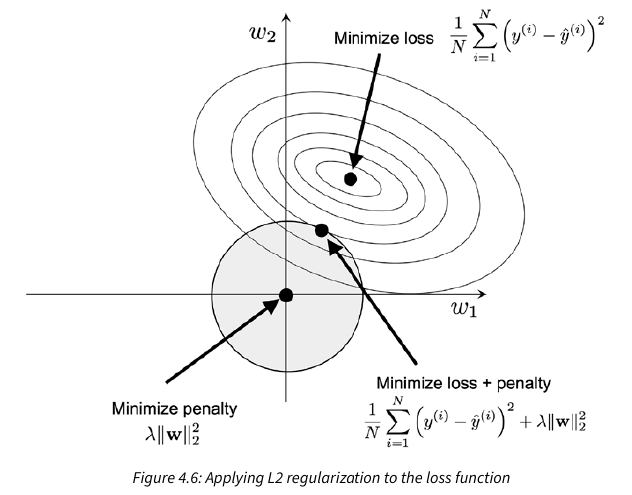
\includegraphics{L2.png}

\vspace{10pt}

Lasso Regression on the other hand tries to minimize the magnitudes. It can lead to many zero values in our coefficients set

%\begin{tikzpicture}
%\node[inner sep=0pt] at (0,0) {\pgfimage[width=10cm]{Courses/images/L1.png}};
%\end{tikzpicture}

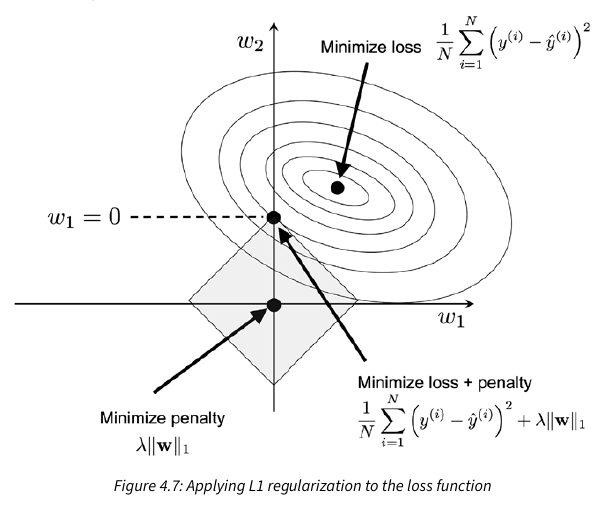
\includegraphics{L1.png}





\hrule



\subsubsection{Lecture 4}

Today we look at our first algorithms, we start with \textbf{Linear Regression}.

\vspace{10pt}

We want to find a relationship between independent variables and the dependent one. The objective is to make predictions based on the past observations.

\vspace{10pt}

As we know one kind of task for ML models is regression, we want to predict a continuous values. One way is using Linear Regression.

The steps are:
\begin{enumerate}
    \item Use least-squares to fit a line on the data
    \item Calculate the $R^2$
    \item Calculate the p-value for $R^2$
\end{enumerate}

A regression model can be simple or multiple

\begin{equation}
    Y = \beta_0 + \beta_1X_1+ \beta_2X_2+...+\beta_nX_n+\varepsilon
\end{equation}

Where:
\begin{itemize}
    \item Y \ra Model/output
    \item $\beta_0$ \ra Intercept
    \item $\beta_n$ \ra Parameters
    \item $X_n$ \ra Inputs
    \item $\varepsilon$ \ra Residuals
\end{itemize}

\vspace{10pt}

For the simple model we only use the first 2 $\beta$ and the first X

We want to minimize the squared sum of the residuals, this will give us a good model. Since this is a minimization problem on both the parameters we differentiate them getting the following formulas (notes that those are estimations)

\begin{equation}
    \hat{\beta_1} = \frac{\Sigma(X_i-\bar{X})(Y_i-\bar{Y})}{\Sigma(X_i-\bar{X})^2}
\end{equation}

\begin{equation}
    \hat{\beta_0} = \hat{Y} - \hat{\beta_1}\bar{X}
\end{equation}

\vspace{10pt}

As said these are estimations, so we want to evaluate how good they are.

Usually we use $R^2$, it explains how much variation in the output can be explained differently from using just the mean.

\begin{equation}
    R^2 = \frac{SS(mean)- SS(fit)}{SS(mean)}
\end{equation}

Where

\begin{itemize}
    \item SS(mean) or SST \ra $\Sigma(y_i-\bar{y})^2$
    \item SS(fit) or SSE = \ra $\Sigma(y_i-\hat{y_i})^2$
\end{itemize}

\vspace{10pt}

We can also do

\begin{equation}
    R^2=\frac{\text{Var(mean) - Var(fit)}}{\text{Var(mean)}}
\end{equation}

Where

\begin{itemize}
    \item Var(mean) = $\frac{\Sigma(y_i-\bar{y})^2}{n}$ = $\frac{SS(mean)}{n}$
    \item Var(fit) = $\frac{\Sigma(y_i-\hat{y}_i)^2}{n}$ = $\frac{SS(fit)}{n}$
\end{itemize}

\vspace{10pt}

Since bigger models with more features will explain more variability we can use the adjusted $R^2$, it will penalize models with a lot of independent variables

\begin{equation}
    \text{Adjusted }R^2 = 1-\frac{(1-R^2)(N-1)}{N-p-1}
\end{equation}

Where
\begin{itemize}
    \item $R^2$ \ra Current $R^2$
    \item N \ra Samples
    \item p \ra Number of independent variables
\end{itemize}

\vspace{10pt}

After that we can check the p-value for each independent variable to check it's statistical relevance, low p-value means high probability that the variable is useful.

\vspace{10pt}

Another model that we have to look at is \textbf{Logistic Regression}, despite the name is a classifier and not a regressor. We want to make a binary classification (1 or 0) based on our data. Differently from the Linear regression loss function (SSE) here we use MLE (Maximum Likelihood Estimation) to maximize the probability of being right.

\vspace{10pt}

Usually our decision is like this

\begin{equation}
    \begin{cases}
        \text{1 \hspace{10pt} if True} \\
        \text{0 \hspace{10pt} if False}
    \end{cases}
\end{equation}

In such cases we can't easily (or we straight up can't) linearly separate those examples, the we need a non linear discriminator with an output between 0 and 1. We want to model the probabilities of being of either class. The function used is a Sigmoid.

\begin{equation}
    p = \frac{1}{1 + e^{-(\beta_0 +\beta_1x)}}
\end{equation}

As said we use MLE to estimate the parameters of the function. Basically we maximise the 
probability of observing the sample.

\vspace{10pt}

Since we want to get a probability between 0 and 1 we have to follow some passages.
\begin{itemize}
    \item We start from the probability \(p = P(Y=1 \mid X)\).
    \item We convert it into \textbf{odds}: \(\dfrac{p}{1-p}\), which range from \(0\) to \(+\infty\).
    \item We take the \textbf{log} of the odds (logit): \(\log\left(\dfrac{p}{1-p}\right)\), which can take any real value \((-\infty, +\infty)\).
    \item We model the log-odds with a \textbf{linear function of the inputs}:  
    \[
    \log\left(\dfrac{p}{1-p}\right) = \beta_0 + \beta_1 x_1 + \dots + \beta_k x_k
    \]
    \item We estimate the parameters \(\beta_0, \beta_1, \dots, \beta_k\) using \textbf{Maximum Likelihood}:  
    each observed \(y_i\) contributes a probability  
    \[
    p_i^{\,y_i} (1 - p_i)^{\,1 - y_i}
    \]
    and we choose the parameters that maximize the likelihood of all observations.
    \item Once the parameters are learned, we plug the linear combination back and convert it to a probability:
    \[
    p = \frac{1}{1 + e^{-(\beta_0 + \beta_1 x_1 + \dots + \beta_k x_k)}}
    \]
    \item This final expression is the \textbf{sigmoid (logistic) function}, which always returns a value between 0 and 1.
\end{itemize}

\vspace{10pt}

To estimate the parameters and how to interpret them:

\begin{itemize}
    \item Parameters are chosen to maximize the likelihood of observing the sample.
    \item Unlike linear regression, there are no closed-form formulas.
    \item We maximize the \textbf{log-likelihood} numerically.
    \item ML estimates are obtained iteratively until the log-likelihood stabilizes.
    \item Predicted log-odds:
    \[
        \hat{y}_i = \hat{\beta}_0 + \hat{\beta}_1 x_{1i} + \dots + \hat{\beta}_k x_{ki}
    \]
    \item Estimated probability:
    \[
        \hat{P}(Y_i=1|X_i) = \frac{e^{\hat{y}_i}}{1+e^{\hat{y}_i}}
    \]
    \item Sign of \(\hat{\beta}_k\) indicates direction of curve:
    \begin{itemize}
        \item \(\hat{\beta}_k > 0\) : probability increases with \(x_k\)
        \item \(\hat{\beta}_k < 0\) : probability decreases with \(x_k\)
    \end{itemize}
    \item Rate of change increases with magnitude of \(\hat{\beta}_k\)
    \item Example: \(\hat{malign}_i = -7.7836 + 0.6683 \cdot thickness + 0.5540 \cdot size + 0.6807 \cdot shape\)
    \begin{itemize}
        \item thickness=5, size=2, shape=2 \(\Rightarrow \hat{P} \approx 0.12\)
        \item thickness=10, size=8, shape=9 \(\Rightarrow \hat{P} \approx 0.999\)
    \end{itemize}
\end{itemize}



\vspace{10pt}

\hrule

\vspace{10pt}

\subsubsection{Lecture 5}

Today we see model selection with Carina Albuquerque (breaking bad mentioned).

We want to find the best model from a set of possible ones. Either comparing different models or different hyperparameters and the same model.

\vspace{10pt}

We want to reduce overfitting, emphasize understanding vs memorizing the data.

This step comes right before the Assessment, so how we check the effective quality of the model.
The main idea of model selection is finding the model that generalizes better on unseen data. Based on the
no free lunch theorem we know that we can't have a ML model that is perfect for every taks. Then we need to accept some trade-offs.

\vspace{10pt}

Since models rely on training data to learn we can encounter the risk that they will memorize those data, this is the case of \textbf{overfitting}.
The other possibility is the one of \textbf{underfitting}, where the model is too rigid and won't learn enough.

\vspace{10pt}

To avoid overfitting we can use different strategies. One of them is splitting the training data into Train and Validation sets. The latter will be used to choose the optimal hyperparameters.
The idea is to minimize the validation error as much as possible. Without a validation set we won't be able to have a good idea on the generalization on unseen data.

\vspace{10pt}

The usual methods employed are
\begin{enumerate}
    \item \textbf{Hold-Out} \ra We take that validation set and we test the model on it
    \item \textbf{K-fold Cross-Validation} \ra We repeat the hold-out k times on different validation sets, stratified version for imbalanced datasets. After the cross-validation we check the performance on the test set. K is usualy equal to 10.
    \item \textbf{Repeated stratified Cross-Validation} \ra Further reduces variance
    \item \textbf{Leave-One-Out Cross-Validation} \ra The cardinality of the validation set is 1
\end{enumerate}


\vspace{10pt}

To compare and choose between two models

\begin{enumerate}
    \item Choose a metric
    \item Choose an evaluation method
    \item Run the mathod for each model
    \item Compare the metrics
    \item Pick the model with the best performance
\end{enumerate}

The best model usually is the simplest, the less prone to error and the one the has the simplest knowledge representation.


\subsubsection{Lecture 6}
















\subsection{Brief recap of models and other useful things}

\subsubsection{Lecture 1}

\begin{itemize}
    \item \textbf{Training example:} A pair $(x, f(x))$.
    \item \textbf{Target function:} The true function $f(x)$ that we want to estimate.
    \item \textbf{Hypothesis:} A proposed function $h$, believed to be similar to $f$; the output of the learning algorithm.
    \item \textbf{Concept:} Boolean function that describes the instances of the dataset.
          \begin{itemize}
              \item $f(x) = 1 \;\Rightarrow$ positive example
              \item $f(x) = 0 \;\Rightarrow$ negative example 
          \end{itemize}
    \item \textbf{Classifier:} A discrete-valued function produced by the learning algorithm.  
          The possible values of $f \in \{1,2,\dots,K\}$ are the \emph{classes} or \emph{class labels}.  
          (In most algorithms the classifier actually returns a real-valued function that must be interpreted).
    \item \textbf{Hypothesis space:} The space of all hypotheses that can, in principle, be produced by the learning algorithm.
    \item \textbf{Version space:} The subset of the hypothesis space that has not yet been ruled out by the training examples.
\end{itemize}


\subsubsection{Lecture 2}
\subsubsection{Lecture 3}
\subsubsection{Lecture 4}
\subsubsection{Lecture 5}

\subsection{Things seen at the practical}

\subsubsection{ML process}

\begin{itemize}
    \item Identify business needs
    \item Import and integrate data
    \item Explore the data
    \item Data preparation
    \item Modelling
    \item Assessment
    \item Deploiment
\end{itemize}


\subsubsection{Feature selection}

\begin{itemize}
    \item Divide the dataset into Training, Test and Validation
    \item Define independent and target variables
    \item Fill the Nans and preprocess the dataset avoiding data leakage.
    \item Filter methods 
    \begin{enumerate}
        \item Setting a Variance threshold
        \item Correlation indices
        \item Statistical Hypothesis Testing
    \end{enumerate}
    \item Wrapper methods
    \begin{enumerate}
        \item Exhaustive feature selection
        \item Forward selection
        \item Backward selection
        \item Stepwise selection
        \item RFE
    \end{enumerate}
    \item Embedded methods
    \item \begin{enumerate}
        \item Regularization (Lasso and Ridge)
        \item Tree-based methods
    \end{enumerate}
\end{itemize}



\subsubsection{Models}

\begin{itemize}
    \item Decision Tree Classifier
    \item Logistic Regression
    \item Support Vector Classifier
    \item Linear Regression (OLS, Lasso, Ridge, ElasticNet)
\end{itemize}


\subsubsection{Metrics}

\begin{itemize}
    \item MAE
    \item $R^2$
    \item Adjusted $R^2$
    \item MSE
    \item RMSE
    \item MedAE
    \item MAPE
    \item ROC curve
    \item AUC
    \item Precision-Recall curve
    \item Macro Evaluation
    \item Micro Evaluation
    \item OVR methods
    \item Weighted metrics
    \item P-values
    \item Confusion matrix
    \item Accuracy
    \item Precision
    \item Recall
    \item F1
\end{itemize}
\section{Statistic for data science}

\subsection{Theory}

\subsubsection{Lecture 1}

Statistics is the approach of answering questions using data. We aim to find rules that are true for a certain population basing our findings on a smaller subset of the mentioned population (sample)

\vspace{10pt}

\textbf{Unit} $\xrightarrow{}$ Basic objrcts on which the data are collected

\textbf{Variable} $\xrightarrow{}$ Characteristics of units that can take different values

\vspace{10pt}

We can have different types of variables
\vspace{10pt}

\textbf{Categorical}
\begin{itemize}
    \item Nominal
    \item Ordinal
\end{itemize}

\textbf{Quantitative}
\begin{itemize}
    \item Discrete
    \item Continuous
\end{itemize}

Our questions involve large \textbf{populations}. Since we can't measure all of the units of them we usually take a subset called \textbf{sample}. Values that concern the sample are called \textbf{statistics} while the ones that concern the whole population are called \textbf{parameters}. 

\vspace{10pt}

We want to estimate in a precise way those parameters basing the computation on the sample.

One of the problems regarding the samples is that those can be biased. To avoid that we want to get a sample that is representative of the population. One way is the use of \textbf{simple random sampling method}.

\textbf{Describing and visualizing data}

We have different ways to describe our data, they depend on multiple factors.

Categorical variables can be described by a proportion



\[
p = \frac{\text{Number in the category}}{\text{Total number}}
\]

To assess how many units share a certain value we can use a \textbf{Bar chart}

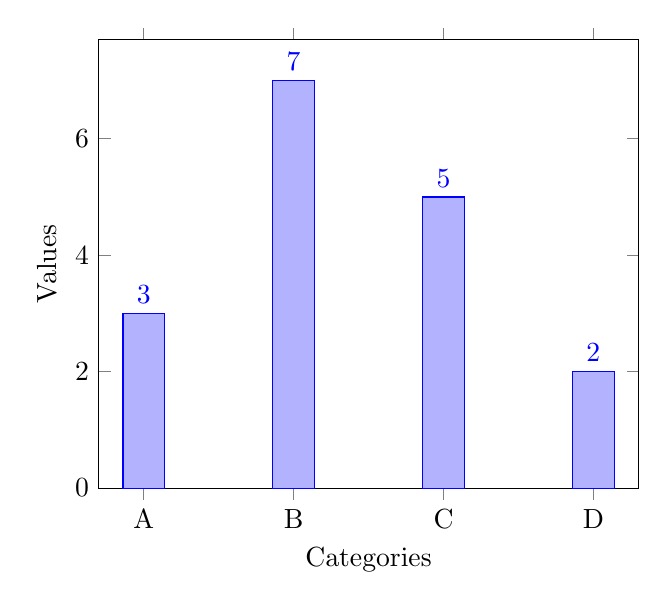
\begin{tikzpicture}
  \begin{axis}[
      ybar,
      bar width=15pt,
      xlabel={Categories},
      ylabel={Values},
      symbolic x coords={A,B,C,D},
      xtick=data,
      nodes near coords, % mostra i valori sopra le barre
      ymin=0,
  ]
    \addplot coordinates {(A,3) (B,7) (C,5) (D,2)};
  \end{axis}
\end{tikzpicture}

\vspace{10pt}

One important concept in statistics is central tendency, which refers to finding the center of our data. It also helps us understand how the other values are distributed around that center. Quantitative variables can be summarized using measures of central tendency.

\vspace{10pt}

\textbf{Mean} $\xrightarrow{}$ Sum of the data values divided by the number of the values. For the mean of the sample we use $\bar{x}$ and for the one of the population $\mu$. The formula is

\[
\bar{x} = \frac{1}{n} \sum_{i=1}^n x_i
\]

\vspace{10pt}

\textbf{Median $\xrightarrow{}$} The center of sample after it was ordered from smallest to largest. Better than mean if we have outliers.

\vspace{10pt}

\textbf{Standard deviation} $\xrightarrow{}$ It describes how the units are distributed from the mean. We can square it to get the variance. For the sample we call it $s$, for the population we use $\sigma$. 

\[
s = \sqrt{\frac{1}{n-1} \sum_{i=1}^n (x_i - \overline{x})^2}
\]

Remember that both $\bar{x}$ and $s$ (or $s^2$) are relative to the sample. They are just an estimation that might be correct if we have a big enough sample.

\vspace{10pt}

\textbf{Percentile} $\xrightarrow{}$ Is a measure that tells us the percentage of the observations that fall at or below it. At $75\%$ we will find on the left the 75\% of the observations and on the right the 25\%.

\vspace{10pt}


\textbf{Quartiles} $\xrightarrow{}$ Basically the same as the percentiles but now we are dividing the sample in 4 parts. $Q_1$ is the first quartile, we will find on the left 25\% of the observations and the rest on the right. $Q_2$ is the median.

\[
Q_1 = \text{25th percentile}, \quad
Q_2 = \text{median (50th percentile)}, \quad
Q_3 = \text{75th percentile}
\]

\[
\text{Interquartile Range (IQR)} = Q_3 - Q_1
\]

\[
\text{Lower fence} = Q_1 - 1.5 \cdot \text{IQR}, \quad
\text{Upper fence} = Q_3 + 1.5 \cdot \text{IQR}
\]

\[
\text{Outliers} = \text{values outside } [\text{Lower fence}, \text{Upper fence}]
\]

\vspace{10pt}

We can visualize those statistics using a \textbf{Boxplot}

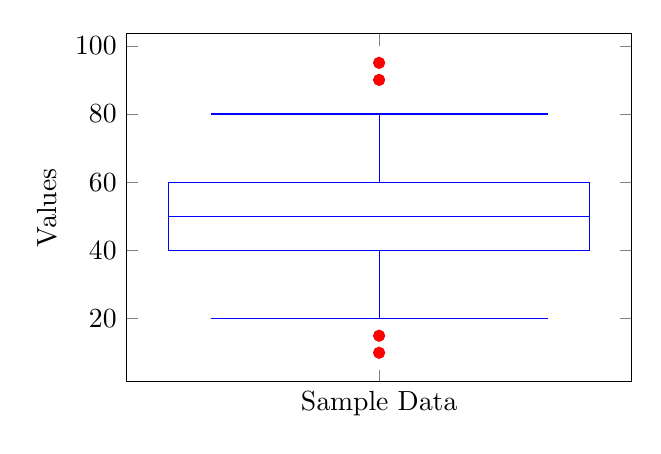
\begin{tikzpicture}
\begin{axis}[
    boxplot/draw direction=y,
    ylabel={Values},
    xtick={1},
    xticklabels={Sample Data},
    width=8cm,
    height=6cm
]

% boxplot principale
\addplot+[
    boxplot prepared={
        median=50,
        upper quartile=60,
        lower quartile=40,
        upper whisker=80,
        lower whisker=20
    },
] coordinates {};

% outlier come punti separati
\addplot+[
    only marks,
    mark=*,
    mark options={red},
] coordinates {(1,10) (1,15) (1,90) (1,95)};

\end{axis}
\end{tikzpicture}



\vspace{10pt}

\textbf{Correlation} $\xrightarrow{}$ Describes the strength and direction between two quantitative variables. For the sample we use $r$, for the population we use $\rho$.

\vspace{10pt}

Correlation has many properties:
\begin{enumerate}
    \item $\rho$ is bounded in [-1, 1]
    \item $\rho$ > 0 means positive association, $\rho$ < 0 negative, $\rho$ = 0 no relationship
    \item The bigger |$\rho$| the stronger the correlation
    \item The sign tells the direction
    \item $\rho$ is unit free
    \item $\rho$(X, Y) = $\rho$(Y, X)
    
\end{enumerate}

To visualize correlation we use a \textbf{Scatterplot}


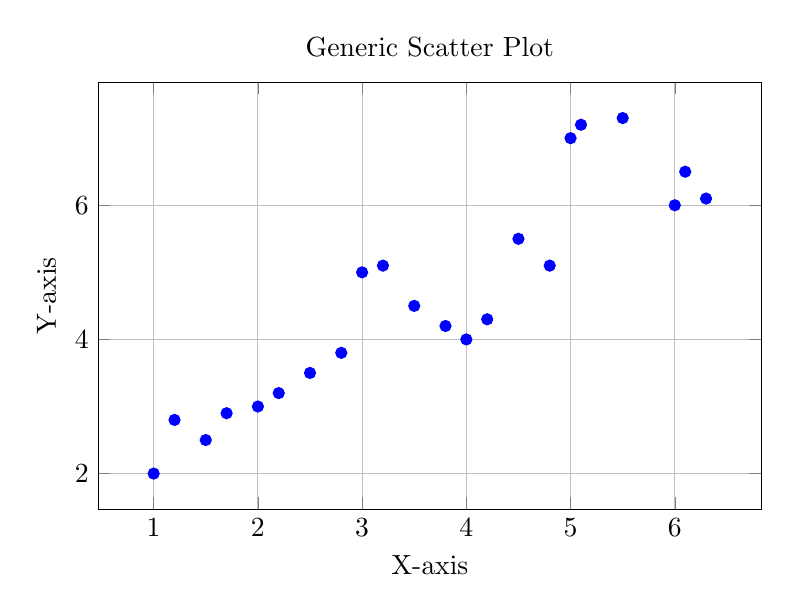
\begin{tikzpicture}
  \begin{axis}[
      xlabel={X-axis},
      ylabel={Y-axis},
      title={Generic Scatter Plot},
      width=10cm,
      height=7cm,
      grid=major,
  ]
    % Dati del scatter plot
    \addplot[
      only marks,
      mark=*,
      mark size=2pt,
      color=blue
    ] coordinates {
        (1,2) (2,3) (3,5) (4,4) (5,7) (6,6)
        (1.5,2.5) (2.5,3.5) (3.5,4.5) (4.5,5.5)
        (1.2,2.8) (2.2,3.2) (3.2,5.1) (4.2,4.3)
        (5.1,7.2) (6.3,6.1) (1.7,2.9) (2.8,3.8)
        (3.8,4.2) (4.8,5.1) (5.5,7.3) (6.1,6.5)
    };
  \end{axis}
  
\end{tikzpicture}

\hrule

\subsubsection{Lecture 2}

\vspace{10pt}

Since random variables can take certain values with certain probabilities we would like to describe them somehow. The collection of those probability is called probability distribution. This can describe the probability of each event happening. Recall that the sum of the probabilities is 1.

\vspace{10pt}

\textbf{CDF} -> the \textbf{cumulative distribution function} gives me the probability that a random variable is less than or equal to a given value. 

\begin{equation}
    F(x) = P(X \le x) \quad \text{for all } x
\end{equation}


\textbf{PMF/PDF} -> the \textbf{probability mass function} or \textbf{probability density function} (for discrete or continuous case respectively) will give us the probability of a certain event happening

\begin{equation}
    f(x) = P(X = x), \quad \text{for all } x
\end{equation}

\begin{equation}
F(x) = \int_{-\infty}^{x} f(t)\,dt, \quad \text{for all } x
\end{equation}

For the continuous case we calculate the integral between the 2 values that we care 

\vspace{10pt}

\textbf{Discrete distributions}

If we can count the sample space we say that our random variable is discrete

Recall

\begin{equation}
    Var[X] = E[X^2] - E[X]^2
\end{equation}

\vspace{20pt}

\textbf{Bernoulli} -> the probability that a certain event will happen

\begin{equation}
    X \sim Ber(p)
\end{equation}
\begin{equation}
    P(X=1) = p = 1 -P(X=0) = 1-q
\end{equation}

With PMF

\begin{equation}
    f(x) = p^x(1-p)^x \quad \text{for x} \in \{0, 1\}
\end{equation}

Where

\begin{itemize}
    \item p -> positive probability
    \item q -> negative probability, 1-p basically
\end{itemize}

And with
\begin{itemize}
    \item E[X] = p
    \item Var[X] = pq = p(1-p)
\end{itemize}


\textbf{Binomial} -> probability of getting a certain number of getting n independent Bernoulli outcome

\begin{equation}
    X \sim Bin(n, p)
\end{equation}

\begin{equation}
    P(X=x) = \binom{n}{x}p^x(1-p)^{n-x}
\end{equation}

Where
\begin{itemize}
    \item n -> number of trials
    \item p -> positive probability
    \item x -> successes that we want to calculate
\end{itemize}

Recall that

\begin{equation}
    \binom{n}{x} = \frac{n!}{x!(n-x)!}
\end{equation}

And with
\begin{itemize}
    \item E[X] = np
    \item Var[X] = np(1-p)
\end{itemize}


\textbf{Poisson} -> probability of getting a certain number of events during a fixed interval. We need to know the probability of the event happening.

\begin{equation}
    X \sim Poi(\lambda)
\end{equation}

\begin{equation}
    f(x) = P(X=x) = \frac{\lambda^xe^{-\lambda}}{x!}
\end{equation}

Where

\begin{itemize}
    \item e -> Euler number
    \item x -> number of successes
    \item $\lambda $ -> known mean rate
\end{itemize}

With
\begin{itemize}
    \item E[X] = Var[X] = $\lambda$
\end{itemize}

\subsubsection{Lecture 3}

\textbf{Continuous distributions}

\vspace{10pt}


\textbf{Normal distribution} -> If we want to describe a series of random events that have a tendency of being near a certain mean.

\begin{equation}
    X \sim N(\mu, \sigma^2
\end{equation}

\begin{equation}
    \phi (x) = \frac{1}{\sqrt{2\pi\sigma^2}} \exp{\{-\frac{1}{2\sigma^2} (x-\mu)^2\}}
\end{equation}

\begin{itemize}
    \item E[X] = $\mu$
    \item Var[X] = $\sigma^2$
\end{itemize}

It has a bell shape and if the parameter are $\mu$ = 0 and $\sigma^2$ = 1 we say that is a standard normal distribution known as Z distribution. $\sigma^2$ will tell us how thin or wide is the distribution, so how variable it is, and so how unpredictable. 

Kurtosis -> Measure of how heavy the tails are, how frequent are the outliers

\vspace{10pt}

\vspace{10pt}

\textbf{Chi squared} -> If we have n independent X variables that are distributed with the Z distribution if we square and sum them we say that this quantity follows a Chi-squared distribution

\begin{equation}
    V=X_1^2+X_2^2+...+X_n^2 \sim\chi_{(n)}^2, n>0
\end{equation}

With
\begin{itemize}
    \item E[V] = n
    \item Var[V] = 2n
\end{itemize}

The n parameter is called \textbf{degrees of freedom}. The shape is asymmetric

\vspace{10pt}


\textbf{Student’s t distribution} $\rightarrow$  
If we have a random variable $Z$ distributed as a standard normal distribution and another independent variable $V$ following a Chi-squared distribution with $n$ degrees of freedom, then the following ratio defines a random variable that follows a t-distribution:

\begin{equation}
    T = \frac{Z}{\sqrt{V / n}} \sim t_{(n)}, \quad n > 0
\end{equation}

With
\begin{itemize}
    \item $E[T] = 0$ \quad (for $n > 1$)
    \item $Var[T] = \dfrac{n}{n - 2}$ \quad (for $n > 2$)
\end{itemize}

The parameter $n$ is called \textbf{degrees of freedom}.  
The distribution is symmetric around zero and has heavier tails than the normal distribution.  
As $n \to \infty$, the t-distribution approaches the standard normal distribution.

\vspace{10pt}


\textbf{Snedecor’s F distribution} $\rightarrow$  
If we have two independent random variables $U$ and $V$ such that  
$U \sim \chi^2_{(n_1)}$ and $V \sim \chi^2_{(n_2)}$,  
then the following ratio defines a random variable that follows an F-distribution:

\begin{equation}
    F = \frac{(U / n_1)}{(V / n_2)} \sim F_{(n_1, n_2)}, \quad n_1, n_2 > 0
\end{equation}

With
\begin{itemize}
    \item $E[F] = \dfrac{n_2}{n_2 - 2}$ \quad (for $n_2 > 2$)
    \item $Var[F] = \dfrac{2n_2^2 (n_1 + n_2 - 2)}{n_1 (n_2 - 2)^2 (n_2 - 4)}$ \quad (for $n_2 > 4$)
\end{itemize}

The parameters $n_1$ and $n_2$ are called \textbf{degrees of freedom} of the numerator and denominator, respectively.  
The distribution is asymmetric and always non-negative.  
It is mainly used to compare variances, especially in the context of ANOVA (Analysis of Variance) and regression models.


\vspace{10pt}

To summarize

\begin{table}[h]
    \centering
    \begin{tabular}{|c|c|c|c|} % '|' crea linee verticali
        \hline % linea orizzontale in alto
        \textbf{Distribution} & \textbf{PDF}  & \textbf{CDF}  & \textbf{Quantile} \\
        \hline % linea sotto l'intestazione
        Normal & dnorm & pnorm & qnorm \\
        \hline
        Chi-Squared & dchisq & pchisq & qchisq \\
        \hline
        Student-t & dt & pt & qt \\
        \hline
        F & df & pf & qf \\
        \hline % linea in fondo
    \end{tabular}
    \label{tab:distributions}
\end{table}

\vspace{10pt}

\hrule

\vspace{10pt}




\subsubsection{Lecture 4}

Today point estimation, hypothesis testing and confidence interval, from a sample we try to generate a good models

\vspace{10pt}

Suppose that we have a population distributed with certain parameters. Like $\mu$ as mean or p as proportion.
Since we can't check the full population (usually), we start from a sample and we try to see if the estimate can be good enough.

\vspace{10pt}

We have two main ways
\begin{itemize}
    \item Method of moments
    \item MLE
\end{itemize}

\vspace{10pt}

To start we need to define the \textbf{Parameter space}, the range of possible values of the parameter $\theta$ inside the oarameter space $\Omega$.
Let $X_1, X_2, ..., X_n$ be n random variables that can take a value $x_1, x_2, ..., x_n$.
The parameter space is bounded.

\vspace{10pt}

To estimate the $\theta$ we use a point estimator. For example the mean is a point estimator of the $\mu$.

\begin{equation}
    \bar{X} = \frac{1}{n} \Sigma X_i
\end{equation}

We define the statistic T($X_1, ..., X_n$) as point estimator to get the parameter estimation.
If T($x_1, ..., x_n$) we get the estimate.


\vspace{10pt}

The first way is the \textbf{Method of moments}, we equate sample moments with theoretical moments.

E($X^k$) is the kth theoretical moment of the distribution, k=1,2,3\dots.

$m_k$ = $ \frac{1}{n} \Sigma X_i^k$

























\subsection{Exercises}  

\begin{itemize}
    \item We have a N$\sim$(102, 8) find the area less than 120

    \begin{verbatim}
        pnorm(120, mean=102, sd=8, lower.tail=TRUE)
    \end{verbatim}

\item Same as above but we want the area more than 120

\begin{verbatim}
    pnorm(120, mean=102, sd=8, lower.tail=FALSE)
\end{verbatim}

\item Proportion of a Z distribution where the z score is between 0 and 1.75

\begin{verbatim}
    pnorm(1.75, mean=0, sd=1, lower.tail=TRUE) - 
    pnorm(0, mean=0, sd=1, lower.tail=TRUE)
\end{verbatim}

\item Proportion of a Z distribution more extreme than $\pm$2

\begin{verbatim}
    pnorm(2, mean=0, sd=1, lower.tail=False)*2
\end{verbatim}

\item Which z-scores separate middle 90\% and the outer 10\%

\begin{verbatim}
    qnorm(0.95, mean=0, sd=1, lower.tail=TRUE)
\end{verbatim}

\item We have a N$\sim$(102, 8), which value separates the top 10\%

\begin{verbatim}
    qnorm(0.90, mean=102, sd=8, lower.tail=TRUE) 
\end{verbatim}

\item Find the 95th percentile of a chi-squared with 7 df

\begin{verbatim}
    qchisq(0.95, df=7)
\end{verbatim}

\item Find 2.5th and 97.5 percentiles of a Student distribution with 5 df

\begin{verbatim}
    qt(0.95, df=5)

    or

    qt(c(0.25, 0.975), df=5)
\end{verbatim}

\item Finde 95th percetile of an F distribution with 12, 5 df

\begin{verbatim}
    qt(0.95, df1=12, df2=5)
\end{verbatim}




\subsection{Code}
    
\end{itemize}


\end{document}
